\section{Generative Adversarial Networks (GANs)}
\label{sec:gan}

\begin{figure}
    \centering
    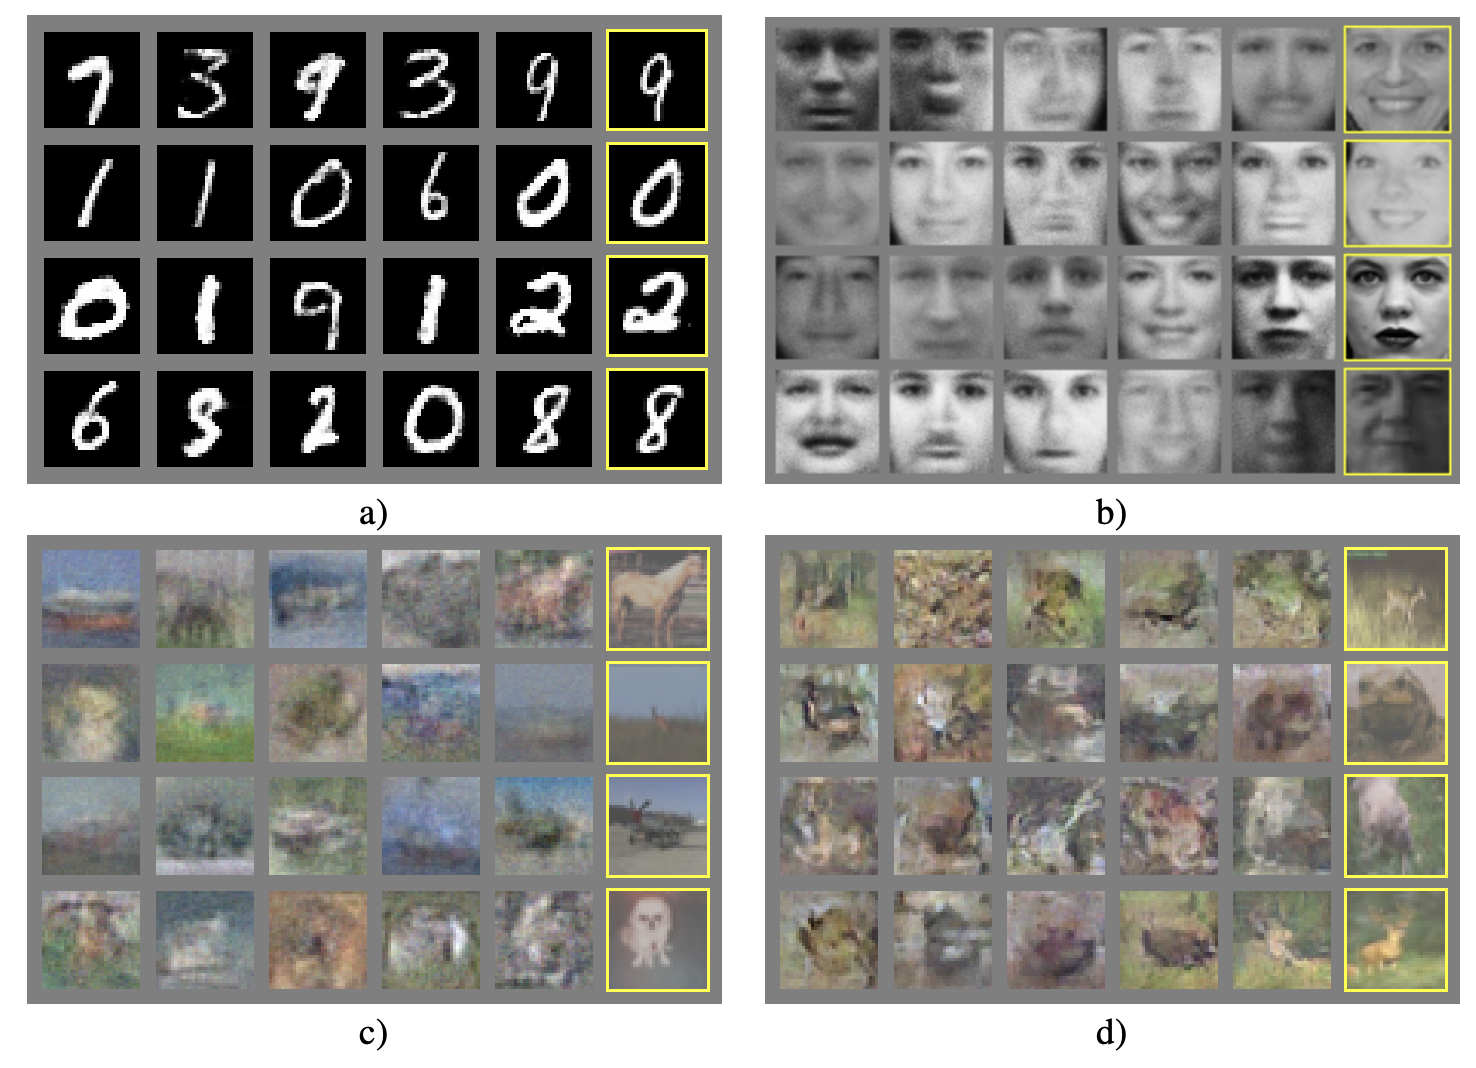
\includegraphics[width=0.6\textwidth]{images/gan/gan_samples.png}
    \caption{Some samples generated by GAN in the paper \cite{gan}. \textit{Yellow column}: samples from the training data which closely resemble the sample to the left \cite{gan}.}
    \label{fig:gan_samples}
\end{figure}

Generative Adversarial Networks (GANs) \cite{gan} are deep learning models that generate new data samples, particularly excelling at synthesizing high-quality images (see figure \ref{fig:gan_samples}). The key innovation is \textbf{adversarial training}, which improves generated image quality through a two-network training approach.

The model comprises two neural networks: a generator $G$ and a discriminator $D$. The generator creates new samples, while the discriminator distinguishes between real and generated samples. They are trained simultaneously in a \textbf{minimax game}, where the generator aims to create indistinguishable samples and the discriminator attempts to detect generated images. 

The input to the generator is a random noise vector $G(z)$ and the output is fake data, which is usually images. The input to the discriminator is either a real or fake data $x$ (fake data generated by the generator) and the output $D(x)$ is a probability that represents the likelihood that the input $x$ is real.

\begin{figure}
    \centering
    \resizebox{\textwidth}{!}{
        \begin{tikzpicture}
            % Real images, Generator nodes
            \node[rectangle, draw, fill=green!20, minimum width=2cm, minimum height=1cm] (real_images) {Real Images};
            \node[rectangle, draw, fill=red!20, minimum width=2cm, minimum height=1cm, below=of real_images] (generator) {Generator};

            % Noise node
            \node[rectangle, draw, fill=gray!20, minimum width=2cm, minimum height=1cm, left=of generator] (noise) {Noise};

            % Arrow from noise to generator
            \draw[->] (noise) -- (generator);

            % Sample nodes
            \node[rectangle, draw, fill=gray!20, minimum width=2cm, minimum height=1cm, right=of generator] (sample_gen) {Sample};
            \node[rectangle, draw, fill=gray!20, minimum width=2cm, minimum height=1cm, right=of real_images] (sample_real_images) {Sample};

            % Fit sample nodes in a box
            \node[fit=(sample_gen)(sample_real_images), inner sep=0] (sample_fitbox) {};


            % Arrows to sample nodes
            \draw[->] (real_images) -- (sample_real_images);
            \draw[->] (generator) -- (sample_gen);

            % Discriminator node
            \node[rectangle, draw, fill=blue!20, minimum width=2cm, minimum height=1cm, right=of sample_fitbox] (discriminator) {Discriminator};

            % Arrows to discriminator
            \draw[->] (sample_real_images) -- (discriminator);
            \draw[->] (sample_gen) -- (discriminator);

            % Discriminator loss, Generator loss
            % Matrix for the nodes to the right
            \matrix[
                right=of discriminator, 
                column sep=0.5cm, 
                row sep=0.5cm, 
                nodes={rectangle, draw, minimum width=4cm, minimum height=2cm, anchor=center}
            ] (matrix) {
                \node[rectangle, draw, fill=gray!20, minimum width=2cm, minimum height=1cm] (discriminator_loss) {Discriminator Loss}; \\
                \node[rectangle, draw, fill=gray!20, minimum width=2cm, minimum height=1cm] (generator_loss) {Generator Loss}; \\
            };

            % Add arrows
            \draw[->] (discriminator) -- (discriminator_loss);
            \draw[->] (discriminator) -- (generator_loss);
        \end{tikzpicture}
    }
    \caption{GAN architecutre \cite{gan}. Noise is sampled from a noise distribution and fed to the generator. The generator outputs an image, and the discriminator needs to decide if the image was generated by the generator or if its an image from the dataset. This decision then affects the value of the loss function, and the weights are updated accordingly by backpropogation.}
    \label{fig:gan_architecture}
\end{figure}

In figure \ref{fig:gan_architecture_highlevel}, noise is sampled from a noise distribution (usually normal distribution) and fed to the generator. The generator outputs an image, and the discriminator decides if the image was generated by $G$ or if it's a sample from the dataset.

\begin{figure}
    \centering
    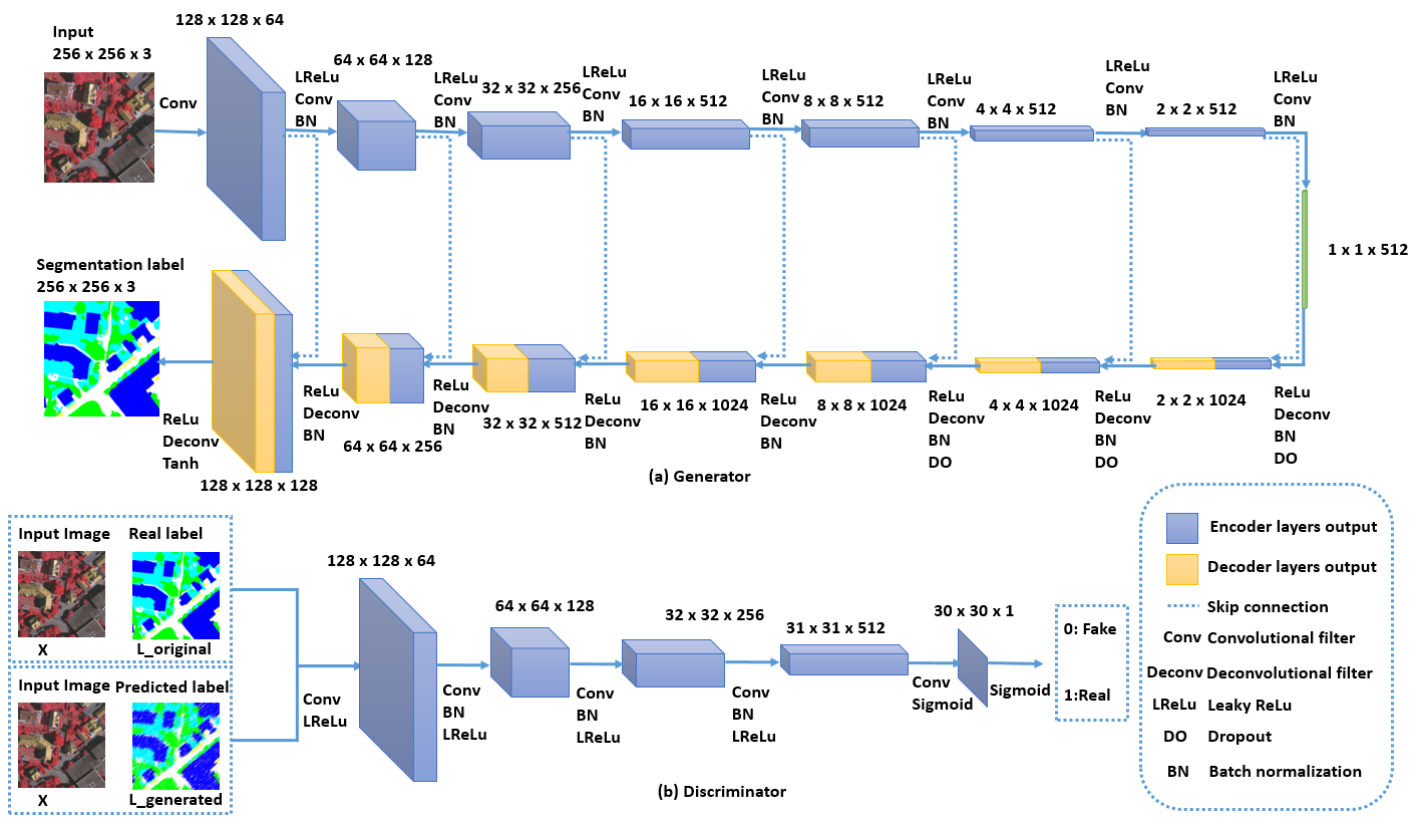
\includegraphics[width=0.8\textwidth]{images/gan/gan_architecture.png}
    \caption{A more detailed architecture of GAN \cite{gan_architecture_figure_paper}. Both the $G$ and $D$ networks are made up of multiple CNN layers. Softmax in $D$ indicates whether the image is real or fake (statistically 1 or 0) \cite{gan_architecture_figure_paper}.}
    \label{fig:gan_architecture}
\end{figure}

Because GANs don't use variational inference like VQ-VAE, the model doesn't have control over the output image: each noise vector will generate a different image. This problem created the need for \textbf{conditional GANs}, which future papers addressed by conditioning the model on additional information (section \ref{subsec:gan_conditional_generation}).




\subsection{Training \& Adversarial loss}
\label{subsec:gan_training}

The GAN loss function is defined as a min-max game:

\begin{equation}
    \label{eq:gan_loss}
    \min_G \max_D V(D,G) = 
    \underbrace{\mathbb{E}_{x \sim p_{\text{data}}(x)}[\log D(x)]}_{\text{real}} + 
    \underbrace{\mathbb{E}_{z \sim p_z(z)}[\log(1 - D(G(z)))]}_{\text{fake}}
\end{equation}

In equation \ref{eq:gan_loss} we have two prior distributions: $x \sim p_{\text{data}}$ and $z \sim p_z(z)$, where the noise vector $z$ is sampled from a noise distribution, and $p_{\text{data}}$ represents the true underlying distribution of the dataset, and $x$ is sampled from this distribution.

The loss function aims to:

\begin{enumerate}
    \item \textbf{The first term}: Maximize the discriminator's ability to correctly classify real samples.
    \item \textbf{The second term}: Minimize the generator's likelihood of producing detectable fake samples.
\end{enumerate}

When we do backpropagation with respect to the generator gradients, the \textbf{first term is constant}.





% \begin{figure}
%     \centering
%     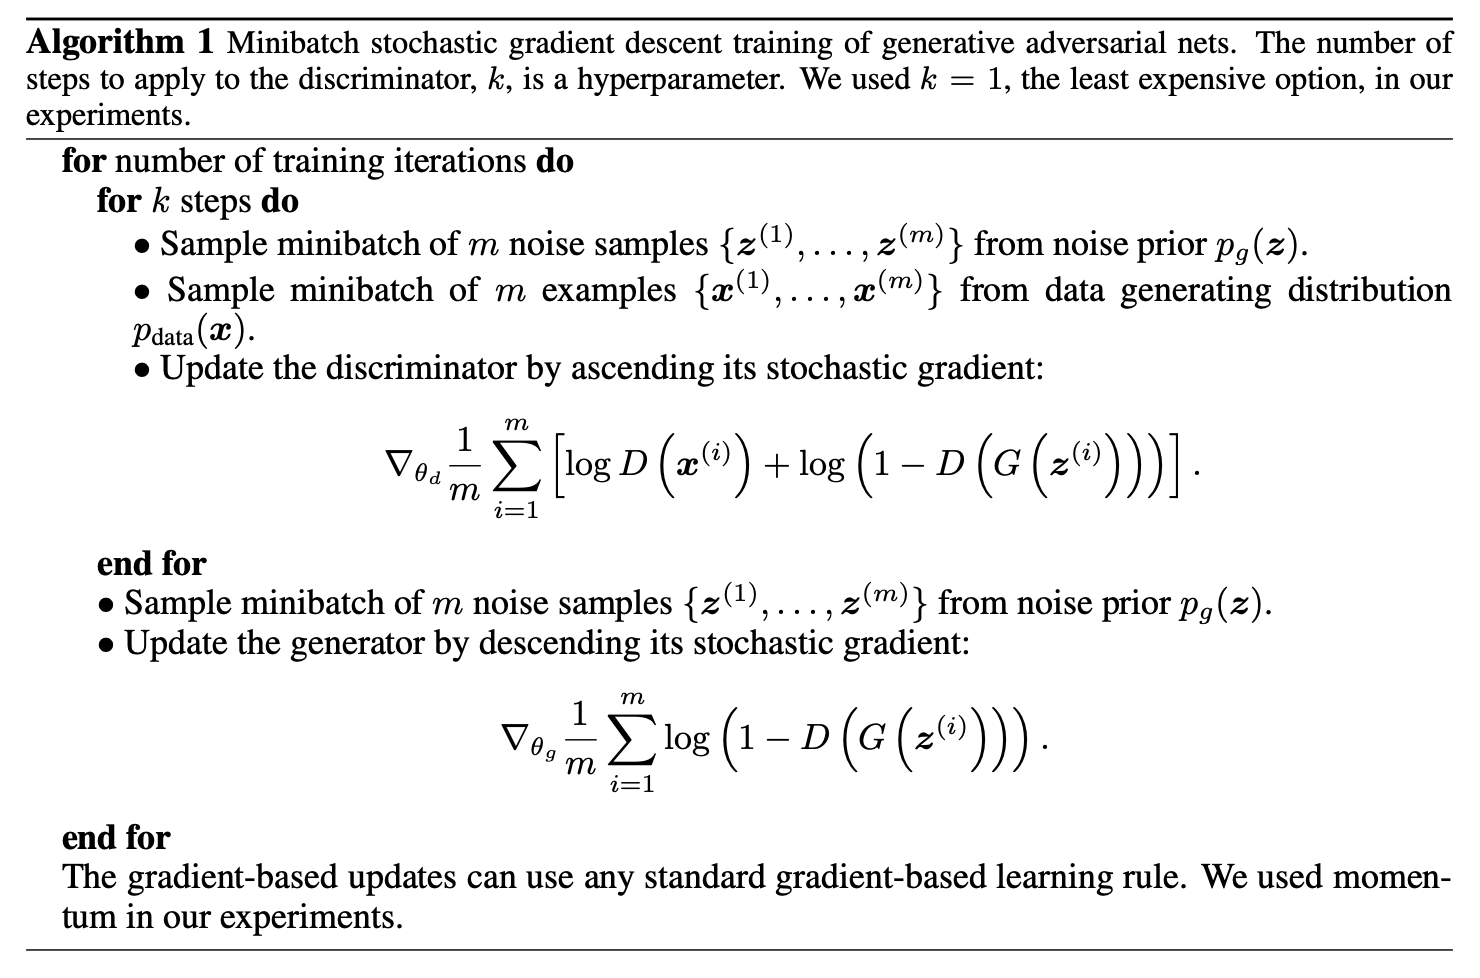
\includegraphics[width=0.7\textwidth]{images/gan/gan_training.png}
%     \caption{The training algorithm for GAN using mini-batch stochastic gradient decent \cite{gan}.}
%     \label{fig:gan_training}
% \end{figure}



\begin{algorithm}
    \caption{The training algorithm for GAN using mini-batch stochastic gradient decent \cite{gan}. The number of steps to apply to the discriminator, $k$, is a hyperparameter. They used $k = 1$, the least expensive option, in their experiments.} 
    \label{alg:gan_training}
    \begin{algorithmic}
        \State \textbf{for} number of training iterations \textbf{do}
        \State \quad \textbf{for} $k$ steps \textbf{do}
        \Statex \qquad $\bullet$ Sample minibatch of $m$ noise samples $\{ \mathbf{z}^{(1)}, \dots, \mathbf{z}^{(m)} \}$ from noise prior $p_g(\mathbf{z})$.
        \Statex \qquad $\bullet$ Sample minibatch of $m$ examples $\{ \mathbf{x}^{(1)}, \dots, \mathbf{x}^{(m)} \}$ from data generating distribution $p_{\text{data}}(\mathbf{x})$.
        \Statex \qquad $\bullet$ Update the discriminator by ascending its stochastic gradient:
        \Statex
        \[
        \nabla_{\theta_d} \frac{1}{m} \sum_{i=1}^{m} \left[ \log D \left( \mathbf{x}^{(i)} \right) + \log \left( 1 - D \left( G \left( \mathbf{z}^{(i)} \right) \right) \right) \right] .
        \]
        \State \quad \textbf{end for}
        \Statex \quad $\bullet$ Sample minibatch of $m$ noise samples $\{ \mathbf{z}^{(1)}, \dots, \mathbf{z}^{(m)} \}$ from noise prior $p_g(\mathbf{z})$.
        \Statex \quad $\bullet$ Update the generator by descending its stochastic gradient:
        \Statex
        \[
        \nabla_{\theta_g} \frac{1}{m} \sum_{i=1}^{m} \log \left( 1 - D \left( G \left( \mathbf{z}^{(i)} \right) \right) \right) .
        \]
        \State \textbf{end for}
    \end{algorithmic}
\end{algorithm}







\textbf{Stabilizing the training}: In order to balance of the training for both $G$ and $D$ the authors suggested using \textbf{iterative approach using mini-batch stochastic gradient decent} (see algorithm \ref{alg:gan_training}). Instead of fully optimizing $D$ in each iteration, the algorithm alternates between a few steps ($k$ steps) of optimizing the discriminator and one step of optimizing the generator.

In algorithm \ref{alg:gan_training} the mini-batch size is $m$. We first sample $m$ noise vectors $z_1, ..., z_m$, and we also sample mini-batch $x_1, ..., x_m$ of size $m$ of the training data distribution $p_\text{data} (x)$. We then \textbf{update the discriminator} $D$ using the formula \ref{eq:gan_loss} (we replaced expectation with sum since we are working in discrete finite space of mini-batch of size $m$, which is why we also divide by $1/m$). Similarly, we sample new noise vectors $z_1, ..., z_m$ and \textbf{update the generator} $G$ using stochastic gradient decent, also similar to formula \ref{eq:gan_loss}. The reason we leave out the term $\mathbb{E}_{x \sim p_{\text{data}}(x)}[\log D(x)]$ in the generator SGD, is because when we do gradient calculation with regard to the generator $G$, this term doesn't have $G$ in it, so it becomes a constant, and we are left with the second term: $\mathbb{E}_{z \sim p_z(z)}[\log(1 - D(G(z)))]$.

Why then we do a for-loop for updating the discriminator and only one update for the generator? Because the researchers wanted to balance the min-max game, and updating the discriminator faster than the prevents the generator from dominating early. However, different implementation can be used: it is possible to update both $G$ and $D$ at the same rate.








\subsection{Mode Collapse}
\label{gan_mode_collapse}

One of the main challenges of training GANs is mode collapse. Mode collapse occurs when the generator learns to generate only a few samples, instead of learning to generate a \textbf{diverse} set of samples. This can happen when the generator focuses only on fooling the discriminator while ignoring to diversify the output samples.

\begin{figure}
    \centering
    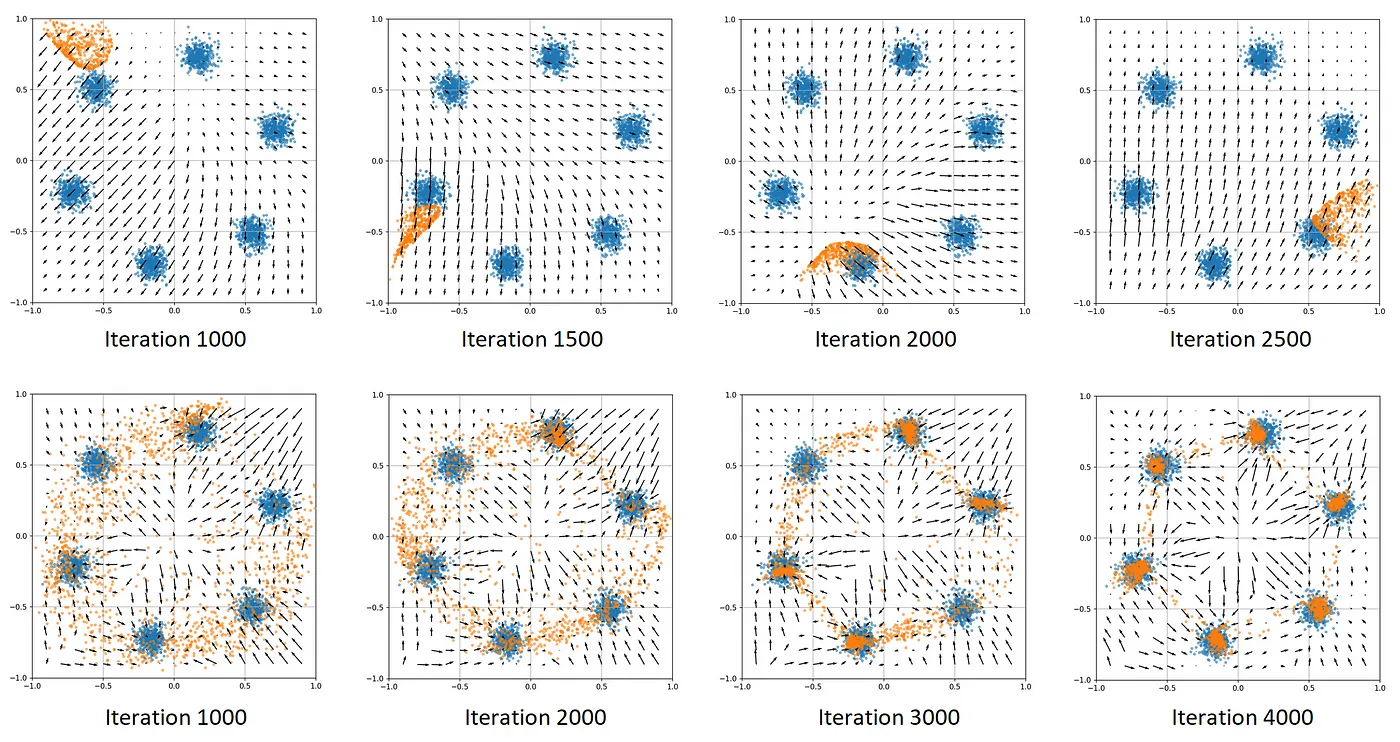
\includegraphics[width=0.6\textwidth]{images/gan/gan_mode_collapse.png}
    \caption{Mode collapse in GANs \cite{gan_mode_collapse_image_source}. \textit{Top row} the model fails to diversify its output, leading it to focus on specific mode of the dataset. \textit{Bottom row}: no mode collapse; the model successfully trained to diversify its output \cite{gan_mode_collapse_image_source}.}
    \label{fig:gan_mode_collapse}
\end{figure}

In figure \ref{fig:gan_mode_collapse} the blue dots are the prior $x \sim p_{\text{data}}(x)$ (the dataset ground truth) and the orange dots are the generated samples $p_g$ by the model.




\subsection{Conditional generation}
\label{subsec:gan_conditional_generation}

Conditional generation models allows to control the output image (style, details, colors and so on). Prominent conditional GAN models include: Conditional GAN (\textbf{cGAN}) \cite{cgan}, \textbf{InfoGAN} \cite{infogan}, \textbf{CycleGAN} \cite{cyclegan}, \textbf{StyleGAN} \cite{stylegan} and more, each with their own unique features and capabilities. 

For example, \textbf{StyleGAN} allows for the control of the style of the generated images by using a separate latent vector for each style. In \textbf{CycleGAN}, the model can learn to translate images from one domain to another without paired data. And in \textbf{InfoGAN}, the model can learn the disentangled latent vectors of the data, which can be used to control the output of the generator (for example, one latent code might control the style of the human head, while another might control the hair color). See figure \ref{fig:gan_conditional_generation} for different examples of conditional generation for InfoGAN and CycleGAN.

\begin{figure}
    \centering
    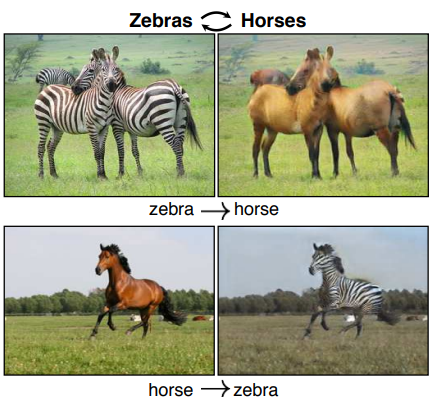
\includegraphics[width=0.3\textwidth]{images/gan/cyclegan.png}
    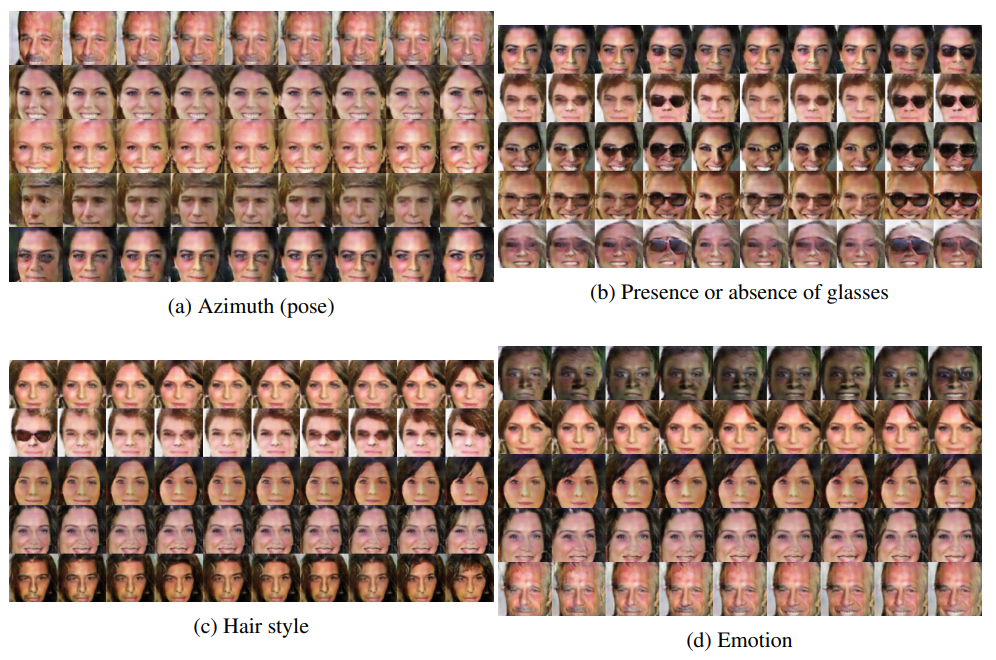
\includegraphics[width=0.5\textwidth]{images/gan/infogan.png}
    \caption{\textit{Left}: \textbf{CycleGAN} can map an image from one distribution to another. \textit{Right}: \textbf{InfoGAN} can be used to control the output (pose, glasses, hairstyle, emotion and more).}
    \label{fig:gan_conditional_generation}
\end{figure}

